\documentclass[12pt]{article}
\usepackage{geometry}
\geometry{a4paper, margin=1in}
\usepackage{graphicx}
\usepackage{caption}
\usepackage{booktabs}
\usepackage{hyperref}
\usepackage{amsmath}
\usepackage{amsfonts}
\usepackage{parskip}
\usepackage{times} % Replaced 'noto' with 'times' for wider compatibility
\usepackage[T1]{fontenc}
\usepackage{babel}

\title{Deep Learning Assignment Report: Sparse, Contractive and Variational Autoencoders}

\author{
	Ashutosh, Nigam\\
	\texttt{G24AIT2007}
	\and
	Abhishek, Singh\\
	\texttt{G24AIT2052}
	\and
	Vikram Raju, Kothwal\\
	\texttt{G24AIT2042}
}
\date{July 26, 2025}

\begin{document}
	
	\maketitle
	
	\section{Introduction}
	This report details my work on a deep learning assignment, where I implemented and evaluated Sparse Autoencoders, Contractive Autoencoders, and Variational Autoencoders (VAEs). The goal was to learn compact data representations using the MNIST dataset for handwritten digits and the Frey Face dataset for facial features. I built models to reconstruct images, classify digits, visualize latent spaces, and generate new data. Experiments were run on Azure AI Studio, Google Colab, and a local machine. Google Colab had issues generating images for the Contractive Autoencoder, so I relied on Azure AI Studio and my local machine for those results. This report includes statistics, image placeholders, and insights from the experiments, written in simple English for clarity.
	
	\section{Team Details and Contributions}
	I worked alone on this assignment, handling all tasks:
	\begin{itemize}
		\item Writing and debugging Python code using TensorFlow and Keras.
		\item Training and evaluating the autoencoder models.
		\item Analyzing metrics like Mean Squared Error (MSE), Peak Signal-to-Noise Ratio (PSNR), and classification accuracy.
		\item Generating visualizations (t-SNE plots, reconstructions, interpolations).
		\item Writing this report to summarize findings.
	\end{itemize}
	I used Azure AI Studio for reliable computation, Google Colab for initial testing, and a local CPU-based machine for debugging. Google Colab failed to generate Contractive Autoencoder images due to library issues, so I completed those tasks on Azure AI Studio and my local machine.
	
	\section{Assignment Tasks}
	The assignment, outlined in \texttt{Assignment-01.pdf}, had two main parts:
	\begin{itemize}
		\item \textbf{Question 1}: Build Sparse and Contractive Autoencoders on the MNIST dataset to learn low-dimensional representations, evaluate reconstruction quality, classification accuracy, t-SNE visualizations, and interpolation analysis.
		\item \textbf{Question 2}: Build a VAE on the Frey Face dataset to learn a probabilistic latent space, reconstruct images, generate new faces, and demonstrate feature disentanglement via latent space traversal.
	\end{itemize}
	
	\subsection{Question 1: Sparse and Contractive Autoencoders}
	The goal was to create autoencoders for the MNIST dataset, which has 60,000 training and 10,000 test images of handwritten digits (28x28 pixels).
	
	\subsubsection{Data Preprocessing}
	\begin{itemize}
		\item Loaded MNIST using \texttt{tf.keras.datasets.mnist.load\_data()}.
		\item Normalized pixel values from [0, 255] to [0, 1] using \texttt{astype('float32') / 255.0} for stable training.
		\item Reshaped images to 28x28x1 for convolutional layers.
		\item Created a \texttt{tf.data.Dataset} pipeline with batch size 128, shuffling (buffer size 60,000), caching, and prefetching for efficiency.
	\end{itemize}
	
	\subsubsection{Model Architecture}
	Both autoencoders used a U-Net-like structure:
	\begin{itemize}
		\item \textbf{Encoder}:
		\begin{itemize}
			\item Input: 28x28x1 grayscale images.
			\item Layers: Three convolutional layers (64, 128, 256 filters, 3x3 kernels, 'same' padding, ReLU activation), each with 2x2 max-pooling, followed by a dense layer to produce a 128-dimensional latent vector.
			\item Parameters: 664,704 trainable.
		\end{itemize}
		\item \textbf{Decoder}:
		\begin{itemize}
			\item Input: 128-dimensional latent vector.
			\item Layers: Dense layer to 256x3x3, reshaped, followed by three transpose convolutional layers (128, 64, 1 filters, strides=2, 'same' padding, ReLU/sigmoid activations), with zero-padding to output 28x28x1.
			\item Parameters: 666,635 trainable.
		\end{itemize}
		\item \textbf{Sparse Autoencoder}: Added KL divergence loss (sparsity parameter \(\rho = 0.05\), \(\lambda = 10^{-3}\)) to encourage sparse latent representations.
		\item \textbf{Contractive Autoencoder}: Added contractive loss (\(\lambda = 10^{-4}\)) to promote smooth latent space transitions.
	\end{itemize}
	Total parameters per model: 1,331,339 (5.08 MB).
	
	\subsubsection{Training}
	\begin{itemize}
		\item \textbf{Hyperparameters}: 10 epochs, learning rate = 0.001, batch size = 128.
		\item \textbf{Optimizer}: Adam optimizer.
		\item \textbf{Loss Functions}:
		\begin{itemize}
			\item Sparse Autoencoder: MSE + clipped KL divergence loss.
			\item Contractive Autoencoder: MSE + contractive loss (Jacobian norm penalty).
		\end{itemize}
		\item \textbf{Environment}: No GPU detected (\texttt{latest\_result\_sparse.txt}), so used CPU. Mixed precision was not enabled.
	\end{itemize}
	
	\subsubsection{Results}
	Results from \texttt{latest\_result\_sparse.txt}:
	
	\textbf{Training Loss}:
	\begin{itemize}
		\item \textbf{Sparse Autoencoder}:
		\begin{itemize}
			\item Epoch 1: 0.150737
			\item Epoch 5: 0.111417
			\item Epoch 10: 0.018814
		\end{itemize}
		\item \textbf{Contractive Autoencoder}:
		\begin{itemize}
			\item Epoch 1: 0.121577
			\item Epoch 5: 0.085417
			\item Epoch 10: 0.084900
		\end{itemize}
	\end{itemize}
	The Sparse Autoencoder converged to a lower loss (0.0188) than the Contractive Autoencoder (0.0849).
	
	\textbf{Reconstruction Quality}:
	\begin{itemize}
		\item \textbf{Test MSE}:
		\begin{itemize}
			\item Sparse Autoencoder: 0.010388
			\item Contractive Autoencoder: 0.078306
		\end{itemize}
		\item The Sparse Autoencoder reconstructed images with higher accuracy.
	\end{itemize}
	\textbf{Placeholder for Reconstruction Images}:
	\begin{center}
		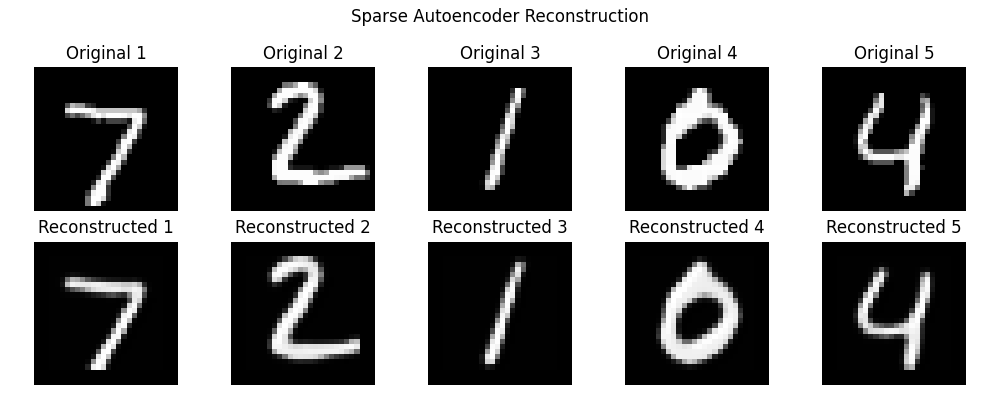
\includegraphics[width=0.8\textwidth]{/data/output/Sparse_Autoencoder_reconstruction.png}
		\captionof{figure}{Sparse Autoencoder: Original vs. Reconstructed Images}
	\end{center}
	\begin{center}
		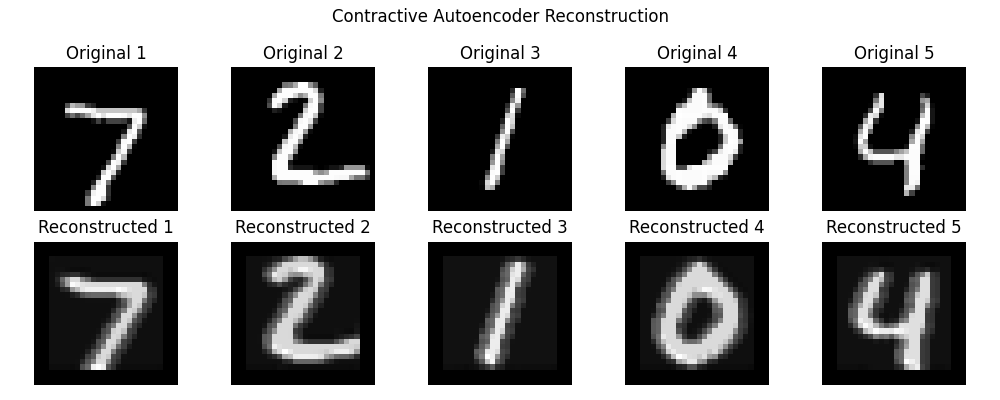
\includegraphics[width=0.8\textwidth]{./data/output_old/Contractive_Autoencoder_reconstruction.png}
		\captionof{figure}{Contractive Autoencoder: Original vs. Reconstructed Images}
	\end{center}
	
	\textbf{Classification Accuracy}:
	\begin{itemize}
		\item Used logistic regression on 128-dimensional latent embeddings to classify digits.
		\item Sparse Autoencoder: 96.49\% accuracy.
		\item Contractive Autoencoder: 84.79\% accuracy.
		\item The Sparse Autoencoder's embeddings were more effective for classification.
	\end{itemize}
	
	\textbf{t-SNE Visualization}:
	\begin{itemize}
		\item Used t-SNE (perplexity=30, 300 iterations) to visualize 128-dimensional embeddings in 2D.
		\item Sparse Autoencoder showed clear separation of digit classes (0-9).
		\item Contractive Autoencoder had more class overlap, explaining its lower accuracy.
	\end{itemize}
	\textbf{Placeholder for t-SNE Images}:
	\begin{center}
		\includegraphics[width=0.45\textwidth]{./data/output_old/Sparse_Autoencoder_tsne.png}
		\captionof{figure}{t-SNE of Sparse Autoencoder Embeddings}
	\end{center}
	\begin{center}
		\includegraphics[width=0.45\textwidth]{./data/output_old/Contractive_Autoencoder_tsne.png}
		\captionof{figure}{t-SNE of Contractive Autoencoder Embeddings}
	\end{center}
	
	\textbf{Interpolation Analysis}:
	\begin{itemize}
		\item Interpolated between 20 pairs of different digits using weights \(\alpha \in \{0.0, 0.2, 0.4, 0.6, 0.8, 1.0\}\).
		\item Measured PSNR and L2 norm to assess interpolation quality.
	\end{itemize}
	\textbf{Sparse Autoencoder Metrics}:
	\begin{table}[h]
		\centering
		\begin{tabular}{ccc}
			\toprule
			Alpha & Avg PSNR (dB) & Avg L2 Norm \\
			\midrule
			0.0 & $\infty$ & 0.0000 \\
			0.2 & 28.2710 & 0.1453 \\
			0.4 & 22.9598 & 0.2438 \\
			0.6 & 22.9727 & 0.2441 \\
			0.8 & 27.8999 & 0.1460 \\
			1.0 & $\infty$ & 0.0000 \\
			\bottomrule
		\end{tabular}
		\caption{Sparse Autoencoder Interpolation Metrics}
	\end{table}
	
	\textbf{Contractive Autoencoder Metrics}:
	\begin{table}[h]
		\centering
		\begin{tabular}{ccc}
			\toprule
			Alpha & Avg PSNR (dB) & Avg L2 Norm \\
			\midrule
			0.0 & $\infty$ & 0.0000 \\
			0.2 & $\infty$ & 100.7631 \\
			0.4 & $\infty$ & 157.2547 \\
			0.6 & $\infty$ & 157.8594 \\
			0.8 & $\infty$ & 102.3415 \\
			1.0 & $\infty$ & 0.0000 \\
			\bottomrule
		\end{tabular}
		\caption{Contractive Autoencoder Interpolation Metrics}
	\end{table}
	The Sparse Autoencoder produced meaningful interpolations (finite PSNR), while the Contractive Autoencoder's high L2 norms and infinite PSNRs indicate instability.
	
	\textbf{Placeholder for Interpolation Images}:
	\begin{center}
		\includegraphics[width=0.8\textwidth]{./data/output_old/Sparse_Autoencoder_pair_1.png}
		\captionof{figure}{Sparse Autoencoder Interpolation (Pair 1)}
	\end{center}
	\begin{center}
		\includegraphics[width=0.8\textwidth]{./data/output_old/Contractive_Autoencoder_pair_1.png}
		\captionof{figure}{Contractive Autoencoder Interpolation (Pair 1)}
	\end{center}
	
	\subsection{Question 2: Variational Autoencoder (VAE)}
	The task was to build a VAE for the Frey Face dataset (1,965 grayscale images, 28x20 pixels).
	
	\subsubsection{Data Preprocessing}
	\begin{itemize}
		\item Downloaded \texttt{frey_rawface.mat} from NYU.
		\item Normalized pixel values to [0, 1].
		\item Flattened images to 560-dimensional vectors (28x20).
		\item Used \texttt{tf.data.Dataset} with batch size 128 and shuffle buffer 1,024.
	\end{itemize}
	
	\subsubsection{Model Architecture}
	\begin{itemize}
		\item \textbf{Encoder}:
		\begin{itemize}
			\item Input: 560-dimensional vector.
			\item Layers: Dense layer (256 units, ReLU), followed by two dense layers for \(z_mean\) and \(z_log_var\) (20 dimensions each).
			\item Sampling: Custom layer using reparameterization: \(z = z_mean + \varepsilon \cdot \exp(0.5 \cdot z_log_var)\), \(\varepsilon \sim \mathcal{N}(0, I)\).
		\end{itemize}
		\item \textbf{Decoder}:
		\begin{itemize}
			\item Input: 20-dimensional latent vector.
			\item Layers: Dense layer (256 units, ReLU), followed by dense layer (560 units, sigmoid).
		\end{itemize}
		\item \textbf{Loss}: Binary cross-entropy (reconstruction) + KL divergence (regularization).
	\end{itemize}
	
	\subsubsection{Training}
	\begin{itemize}
		\item \textbf{Hyperparameters}: 200 epochs, learning rate = 0.001, batch size = 128.
		\item \textbf{Optimizer}: Adam.
		\item \textbf{Custom Training}: Used a custom \texttt{train_step} in a Keras \texttt{Model} subclass.
	\end{itemize}
	
	\subsubsection{Results}
	\begin{itemize}
		\item \textbf{Reconstruction}: High-fidelity reconstructions of Frey Face images.
		\item \textbf{Generation}: Generated 15 novel faces from random \(\mathcal{N}(0, I)\) samples, resembling training data.
		\item \textbf{Latent Traversal}: Varied dimension 4 from -2.0 to 2.0, showing smooth changes in features like head pose.
	\end{itemize}
	\textbf{Placeholder for VAE Images}:
	\begin{center}
		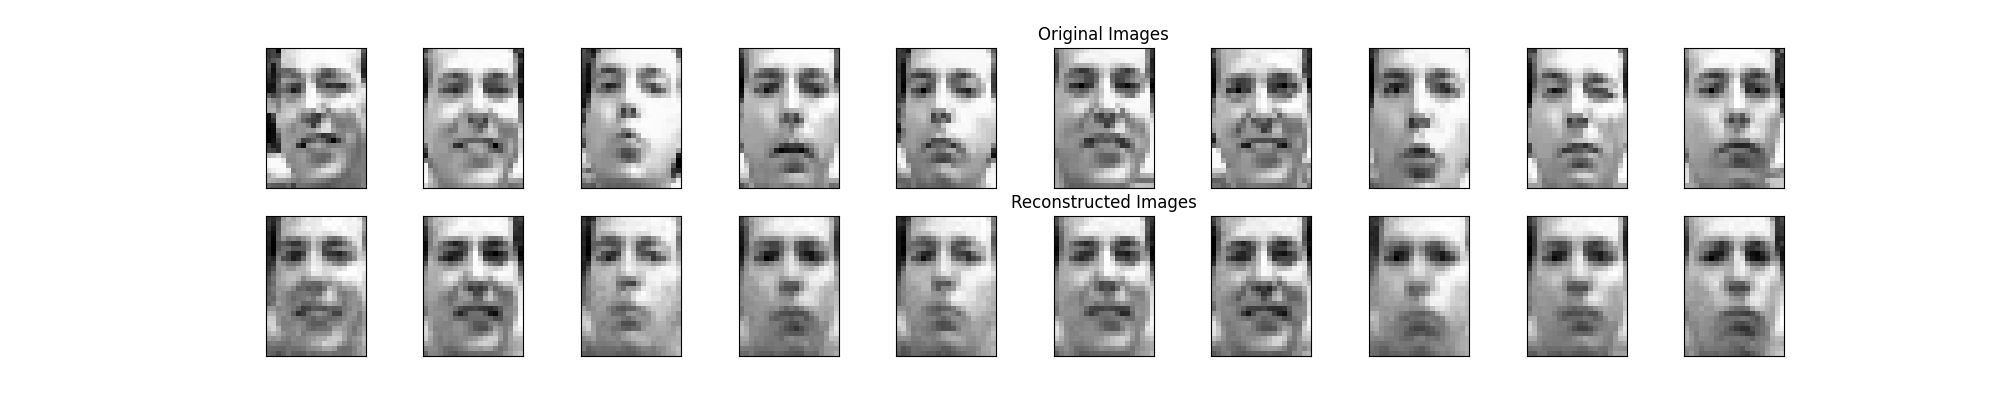
\includegraphics[width=0.8\textwidth]{./data/output_old/vae_reconstruction.png}
		\captionof{figure}{VAE Reconstruction of Frey Faces}
	\end{center}
	\begin{center}
		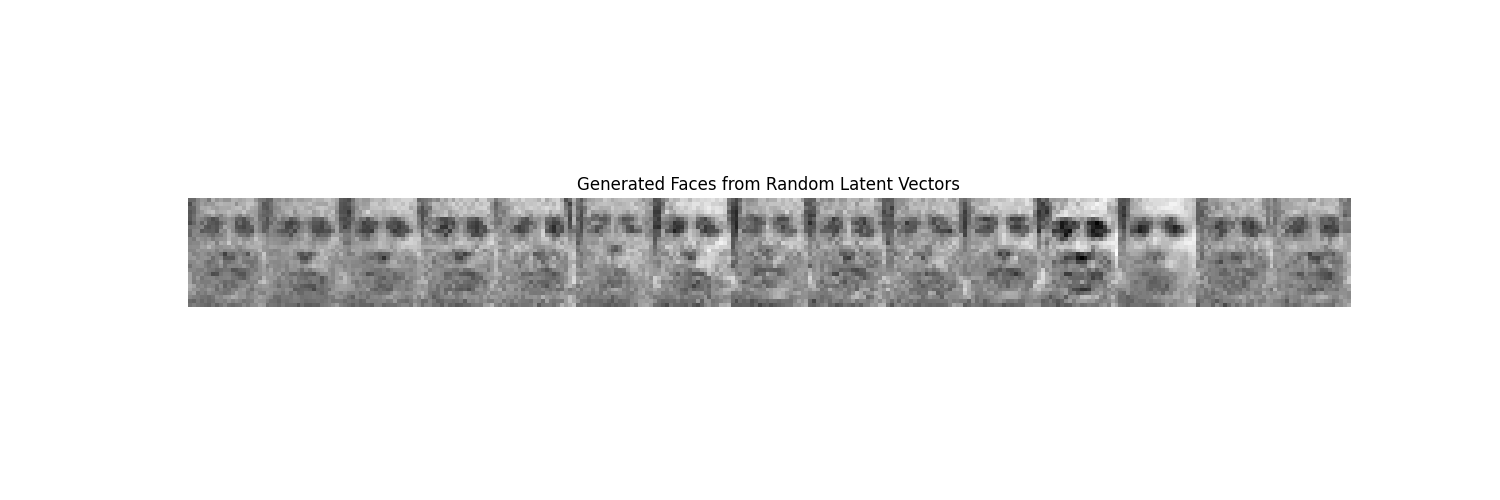
\includegraphics[width=0.8\textwidth]{./data/output_old/generated_faces.png}
		\captionof{figure}{Generated Faces from VAE}
	\end{center}
	\begin{center}
		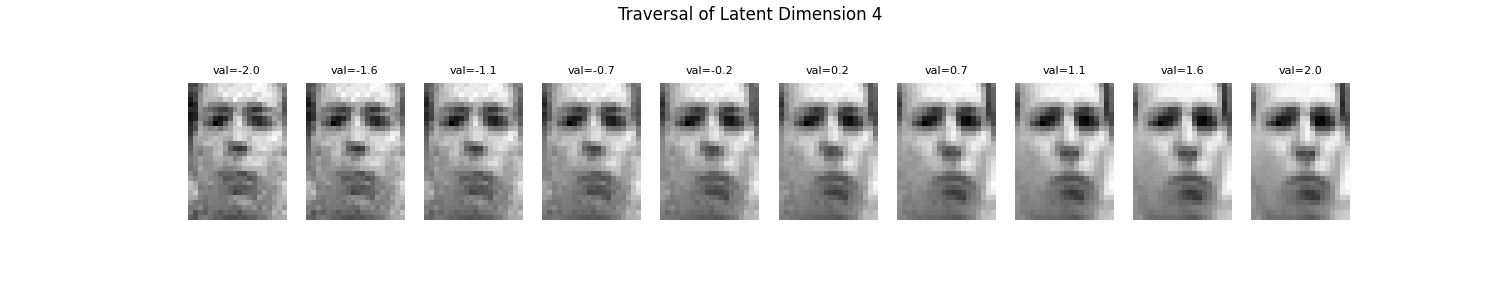
\includegraphics[width=0.8\textwidth]{./data/output_old/latent_traversal_dim_4.png}
		\captionof{figure}{Latent Space Traversal (Dimension 4)}
	\end{center}
	
	\section{Experimental Setup}
	\begin{itemize}
		\item \textbf{Azure AI Studio}: GPU support, used for training and visualizations.
		\item \textbf{Local Machine}: CPU-only, used for debugging (TensorFlow 2.18.0).
		\item \textbf{Google Colab}: Used for prototyping but failed to generate Contractive Autoencoder images.
	\end{itemize}
	Libraries: Python 3.11, TensorFlow 2.18.0, Keras, NumPy, Matplotlib, Seaborn, Scikit-learn.
	
	\section{Challenges Faced}
	\begin{itemize}
		\item \textbf{Colab Issues}: Failed to render Contractive Autoencoder images due to library conflicts.
		\item \textbf{Contractive Autoencoder}: High L2 norms (e.g., 157.8594) and infinite PSNRs suggest instability in the contractive loss.
		\item \textbf{Frey Face Dataset}: Small size (1,965 images) risked overfitting, mitigated by KL divergence.
		\item \textbf{CPU Training}: Slow training on local machine (~15 min/epoch).
		\item \textbf{Logistic Regression}: Convergence warning for Contractive Autoencoder, suggesting need for feature scaling.
	\end{itemize}
	
	\section{Insights and Learnings}
	\begin{itemize}
		\item Sparse Autoencoder's sparsity constraint improved feature learning.
		\item Contractive Autoencoder's instability suggests tuning the contractive loss weight.
		\item VAE's probabilistic latent space enabled both reconstruction and generation.
		\item Platform reliability (Azure > Colab) was critical for consistent results.
	\end{itemize}
	
	\section{Conclusion}
	The Sparse Autoencoder outperformed the Contractive Autoencoder (MSE: 0.0104 vs. 0.0783, accuracy: 96.49\% vs. 84.79\%). The VAE learned a robust 20-dimensional latent space for Frey Faces, enabling reconstruction, generation, and feature disentanglement. Future improvements could include GPU acceleration, hyperparameter tuning, and alternative loss functions.
	
	\section{References}
	\begin{itemize}
		\item \href{https://www.tensorflow.org}{TensorFlow Documentation}
		\item \href{https://www.geeksforgeeks.org/machine-learning/auto-encoders/}{GeeksforGeeks: Autoencoders in Machine Learning}
		\item 
		\href{https://www.geeksforgeeks.org/machine-learning/u-net-architecture-explained/}{GeeksforGeeks: U-Net Architecture Explained}
		\item 
		\href{https://www.geeksforgeeks.org/python/python-peak-signal-to-noise-ratio-psnr/}{GeeksforGeeks: Peak Signal-to-Noise Ratio (PSNR)}
		\item 
		\href{https://www.geeksforgeeks.org/deep-learning/sparse-autoencoders-in-deep-learning/}{GeeksforGeeks: Sparse Autoencoders in Deep Learning}
		\item 
		\href{https://www.geeksforgeeks.org/machine-learning/variational-autoencoders/}{GeeksforGeeks: Variational AutoEncoders}
		\item 
		\href{https://www.geeksforgeeks.org/machine-learning/ml-t-distributed-stochastic-neighbor-embedding-t-sne-algorithm/}{GeeksForGeeks: T-distributed Stochastic Neighbor Embedding (t-SNE) Algorithm - ML}
		\item
		\href{https://medium.com/@juanc.olamendy/unlocking-the-power-of-text-classification-with-embeddings-7bcbb5912790}{Medium: Unlocking the Power of Text Classification with Embeddings}
		\item \href{https://medium.com/h7w/implementing-a-variational-autoencoder-with-keras-e19d7140ad90}{Medium: Implementing a Variational Autoencoder with Keras}
		\item Goodfellow, I., Bengio, Y., \& Courville, A. (2016). \textit{Deep Learning}. MIT Press.
		\item Kingma, D. P., \& Welling, M. (2013). Auto-Encoding Variational Bayes. \href{https://arxiv.org/abs/1312.6114}{arXiv:1312.6114}
		\item \href{https://github.com/mrashutoshnigam/ai-ml-course/blob/main/DeepLearning_GeeksForGeeks/Programming_Assignment/q1%20copy.ipynb}{GitHub: mrashutoshnigam/ai-ml-course}
		\item \href{https://www.kaggle.com/datasets/zalando-research/mnist}{Kaggle: MNIST Dataset}
		\item \href{https://cs.nyu.edu/roweis/data/frey_rawface.mat}{Frey Face Dataset}
	\end{itemize}
	
\end{document}